\chapter{Import \& Export}

\section{Import}
MDL files are imported by selecting \menu{File > Import > Aurora (.mdl)} In the File Selector, 
select a \textit{mdl} file. The following options are available for this add-on: 

\begin{description}[leftmargin=13em,style=nextline]
    \item[Import Geometry] Import the geometry from the mdl file. This may be disabled to only import animations to an already existing model.
    \item[Import Walkmesh] Attempt to import a walkmesh. If the imported model is a placeable, the script will look for a {\textit{pwk}} file in the same folder. If the model is a door, it will look for a {\textit{dwk}} file. If the model is a tile, it will read the walkmesh directly from the \textit{mdl} file.
    \item[Import Smooth Groups] Import smoothing groups as sharp edges.
    \item[Import Animations] Import animations from the mdl file. By default animations will be added to the imported geometry. If no geometry was imported, the script will try to add animations to already existing objects in blender.
    \item[Materials] None = No materials or textures will be imported. Single = Neverblender will attempt to merge similar materials to reduce clutter. Multiple = Each object will get it's own material, even if this results in multiple identical materials.
    \item[Image Search] Search for textures in sub-directories. This might take a significant amount of time depending on the number of files.
\end{description}

\begin{figure}[hb]
    \centering
    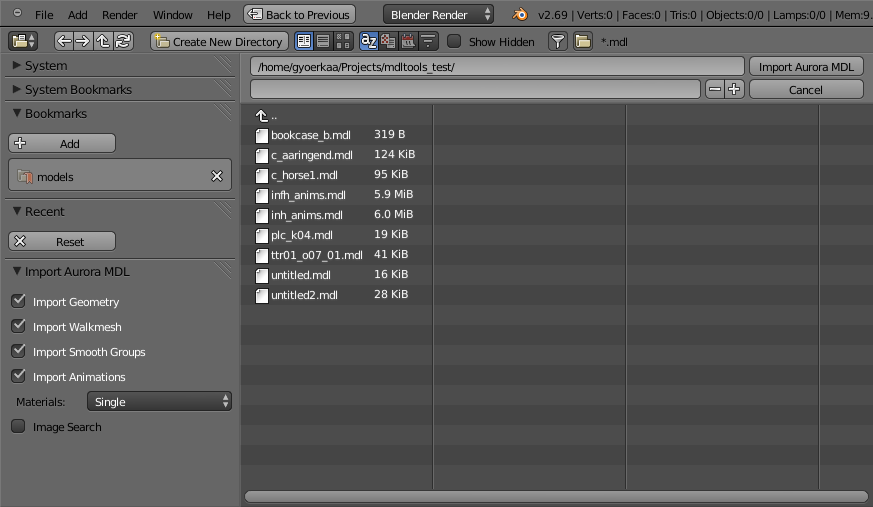
\includegraphics[width=0.9\linewidth]{window_io_import}
    %\caption[Close up of \species{Hemidactylus}]
    %{Close up of \species{Hemidactylus}, which is part the genus of the gecko family. It is the second most speciose genus in the family.}
\end{figure}

\section{Export}
MDL files are exported by selecting \menu{File > Export > Aurora (.mdl)}. If there are multiple MDLs in the scene,
select a part of the one you wish to export - any object will suffice. Select the file name for the mdl. Note that the 
file must have the same name as the Rootdummy. The following options are available for this add-on: 

\begin{description}[leftmargin=12em,style=nextline]
    \item[Export Animations] Export animations to mdl.
    \item[Export Walkmesh] Attempt to export a walkmesh. The type of the exported walkmesh depends on the models classification.
    \item[Export Smooth Groups] Generate smoothing groups. Method depends on the settings of each mesh.
    \item[Apply Modifiers] Apply modifiers before exporting.
\end{description}

\begin{figure}[hb]
    \centering
    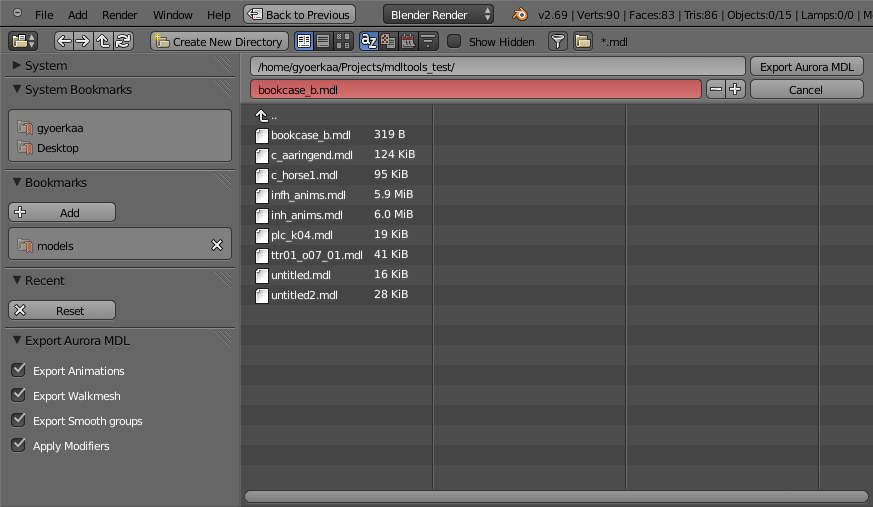
\includegraphics[width=0.9\linewidth]{window_io_export}
    %\caption[Close up of \species{Hemidactylus}]
    %{Close up of \species{Hemidactylus}, which is part the genus of the gecko family. It is the second most speciose genus in the family.}
\end{figure}
